\documentclass[12pt,a4paper]{article}
\usepackage[utf8]{inputenc}
\usepackage[english]{babel}
\usepackage{enumerate}
\usepackage{amsmath}
\usepackage{amsfonts}
\usepackage{amssymb}
\usepackage{graphicx}
\usepackage{fourier}
\usepackage[left=2cm,right=2cm,top=2cm,bottom=2cm]{geometry}
\usepackage{commath}
\usepackage{cancel}
\usepackage{placeins}
%\author{Juan Carlos Apitz, ID 012523821}
%\title{Feature Selection Via Logistic Elastic Net Regression in Genetic Cancer Research}

\begin{document}


\begin{titlepage}
	\centering
	%\includegraphics[width=0.15\textwidth]{example-image-1x1}\par\vspace{1cm}
	{\scshape\Large Feature Selection Via Logistic Elastic Net Regression in Genetic Cancer Research \par}
	\vspace{1cm}
	{\scshape\large A PROJECT REPORT\par}
	%\vspace{1.5cm}
	{\large Presented to Department of Mathematics and Statistics California State University, Long Beach\par}
	\vspace{4cm}
	{\large In Partial Fulfillment of the Requirements for the Degree Master of Science in Mathematics Option in Statistics\par}
	\vspace{3cm}
	{\large Faculty Reviewer:\par}
	\vspace{0.5cm}
	{\large Kagba Suaray, Ph.D.}
	\vfill
	\large By ~Juan Carlos Apitz\\
	\large M.S., 2016, California State University, Long Beach\par

	\vfill

% Bottom of the page
	{\large \today\par}

\end{titlepage}

\tableofcontents

\pagebreak

\begin{abstract}
The purpose of this analysis is to present and implement an effective methodology for dealing with datasets where the number of samples $n$ is much smaller than the number of covariates $p$. This methodology is called regularized logistic regression via the Elastic Net. Having $p>>n$ is a problem common with microarray expression data where typically the dataset contains tens to maybe less than a few hundred samples vs. thousands of genes. A typical problem in this context is that of classification. The response variable in the dataset is typically binary, encoding the presence of a particular cancer class. In our case study we analyze breast cancer expression data containing luminal vs. non-luminal breast cancer types. By implementing the proposed methodology we are able to reduce the number of genes from 47,293 to 1,182 genes. We use the fitted model to perform classification and obtain accuracy of 86\%.
\end{abstract}



\pagebreak

\nocite{*}

\section{Introduction}
A common problem encountered in the analysis of microarray data is high dimensionality. High dimensionality is most acute when the data consists of a few samples (the $n$ dimension) and a large number of explanatory variables (the $p$ dimension). Occam's Razor states that among several plausible explanations for a phenomenon, the simplest is best. Many genes in microarray data are not necessarily relevant to the analysis and simply add noise. There exist many methods to deal with this problem, however some of these methods, such as stepwise reduction may simply not work in situation where the number of relevant genes is still greater than the number of samples.\\
\par In this analysis, we implement a relatively new method: elastic net regularization, combined with logistic regression to reduce the dimensiionality of a breast cancer gene expression dataset and perform classification of cancer types. We will demonstrate the accuracy of this method in classifying cancer types as well as its ability to select a number of explanatory variables (genes in our case) that is much greater than the number of samples. 
\section{The Curse of Dimensionality: When $\mathbf{p>>n}$}
\par A wide variety of interesting problems, specially in fields such as genomics and computational biology \cite{friedman2001elements} , yield data sets where the number of observations is much smaller than the number of covariates that a researcher may wish to consider. For example, this is the standard case for micro-array data sets which typically consist of a few hundreds experimental observations that measure gene expression levels for thousands of genes.\\
\par When $p>>n$ applying the standard methods for solving the ordinary least squares (OLS) problem is not reliable because in this context there are insufficient degrees of freedom to estimate the full model. In other words, the solution $\mathbf{\hat{\boldsymbol{\beta}}=\left(X^\top X\right)^{-1}X^\top Y}$ to the minimization problem $\underset{\boldsymbol{\beta}}{\text{min}} \mathbf{\|Y - X\boldsymbol{\beta}\|^2}$ is not unique. We can find infinitely many  hyperplanes that can fit the lower dimensional set of observation points. As a result the standard OLS solution lacks the information required to estimate all the parameters in the model. Thus, given the high dimemsionality the observed data is said to be a sparse signal. \\
\par One of the most popular approaches to dealing high dimensionality is regularization via the least absolute shrinkage and selection operator (LASSO) developed by Tibshirani in 1996 \cite{tibshirani1996regression}. Under this approach, the OLS problem solution estimates are obtained by minimizing the residual squared error subject to the constraint:
\begin{equation} \label{eq:1} 
\left\|\boldsymbol{\beta}\right\|_1 < t
\end{equation}
where $\boldsymbol{\beta}$ is the vector of OLS coefficients and $t \geq 0$ is a tuning parameter. \\
\par The motivation for the LASSO is two fold: First, it improves prediction accuracy. OLS parameter estimates tend to be unbiased but can have large variance, thus prediction accuracy can be improved by shrinking or setting some coefficients to zero \cite{tibshirani1996regression}. Second, it can be used as a method for variable selection to isolate the most influential subset of variables. The LASSO is an improvement over another two standard methods used to improve OLS estimation: Ridge Regression and Subset Selection methods such as Stepwise Selection. Ridge Regression, being a continuous penalty does not shrink the coefficients all the way to zero, and Subset Selection can be highly sensitive to changes in the data, which makes it unstable. \\
\par The LASSO, however has some shortcomings in the context where $p>>n$ . First the LASSO can only select at most $n$ predictors, a limiting feature for a variable selection method. Second, if a group of predictors is highly correlated, the LASSO will indiscriminately select only one variable from the group. Third, when the predictors are highly correlated, the LASSO performs worse at prediction than Ridge Regression \cite{friedman2001elements}.\\
\par A more effective regularization method for the $p>>n$ situation, specially when the predictors are highly correlated, is the elastic net penalty. This methodology was developed by Zou and Hastie in 2005 \cite{zou2005regularization} and unlike the LASSO it is not limited to selecting at most n predictors. The elastic net penalty incorporates a convex combination of both the LASSO and the Ridge regression penalties:
\begin{equation} \label{eq:2}
\left(1-\alpha\right)\left\|\boldsymbol{\beta}\right\|_1 + \alpha \left\|\boldsymbol{\beta}\right\|_2
\end{equation}
where $0 \leq \alpha \geq 1$. In addition to not having the limitation of selecting at most $n$ predictors, the elastic net has better prediction performance than the LASSO in the presence of highly correlated predictors. This proves particularly important when working with microarray data since the variable genes tend to exhibit strong pairwise correlations. The elastic net regularization can be implemented with most linear classifiers. In the next section we discuss the implementation of elastic net regularized logistic regression and subsequently present a case study in classification with microarray data. 
\section{Classification and Gene Selection in Cancer Genomics}
\subsection{The Naderi et al Breast Cancer Microarray Dataset}
The dataset analyzed in this study is a public breast cancer microarray dataset made available by Naderi et al \cite{naderi2007gene}. It consists of 84 luminal and 44 non-luminal cancer sub-type samples and 47,293 genes. The data represents expression measures for each sample across all 47,293 genes. This dataset is a classic case of $p>>n$ and the remaining of this analysis we will construct a regularized logistic regression model which performs sub-type classification (luminal vs. non-luminal) and significant gene-group selection.
\begin{table}
\begin{center}
\begin{tabular}{|l|c|c|c|}
\hline Value & Count & Frequency/Mean & Std\\
\hline luminal & 84 & 0.65625 & na\\
\hline non-luminal & 44 & 0.34375 & na\\
\hline gene expression & 47,293 & 6.0305 & 0.8214\\
\hline
\end{tabular}
\end{center}
\end{table}

\begin{table}
\begin{center}
\begin{tabular}{|c|c|c|c|c|c|}
\hline RESPONSE & GI-10047089-S & GI-10047091-S & GI-10047093-S\\
\hline luminal & 5.3416 & 5.8460 & 6.7052\\
\hline luminal & 5.6259 & 5.8742 & 6.8089\\
\hline luminal & 5.6181 & 5.8026 & 6.6975\\
\hline
\end{tabular}
\caption{Dataset summary and example of three rows (samples) by three columns (genes).}
\label{table:1}
\end{center}
\end{table}
\par Table \ref{table:1} shows a summary of the data and a 3 X 3 example so the reader can have a visual idea of what the data looks like.

\subsection{Regularized Logistic Regression}
Classifying microarray samples according to whether the sample is from a cancer sub-type is a valuable tool for researchers who seek to understand the relationships between gene expresion levels and cancer.\\
\par In order to classify tissue samples we construct a logistic regression model that produces an estimate of the probability that a given sample comes from the luminal or non-luminal type. In addition to estimating a sub-type probability, this model provides a methodology to perform gene selection. That is, we can use the model to extract the most significant genes in the experiment.\par
The appeal of constructing a logistic regression model arises from the convenience of estimating a probabilistic measure of classification. In logistic regression for a binary variable, we model the natural log of the odds ratio as:
\begin{equation} \label{eq:3}
\log\left(\text{odds}\right) = \log \dfrac{P\left(Y = 1 | X = x\right)}{P\left(Y = 0 | X = x\right)} = \beta_0 + \beta^T x.
\end{equation}
In this study we formulate a random variable $Y$ that equals 1 if the sample came from a luminal type tumor and 0 otherwise. The term in the numerator of equation (\ref{eq:3}) is the probability that a given sample of the luminal type ($Y = 1$). The term in the denominator represents the probability that the sample came from the non-luminal type ($Y = 0$). Mathematically we can express these probabilities as:
\begin{gather} 
\label{eq:4} P\left(Y = 1 | X = x\right) = \dfrac{e^{\beta_{0} + \beta^T x_i}}{1+e^{\beta_{0} + \beta^T x_i}}\\
\label{eq:5} P\left(Y = 0 | X = x\right) = \dfrac{1}{1+e^{\beta_{0} + \beta^T x_i}}.
\end{gather}
Based on this framework we can express the expectation of $Y$ as \cite{nachtsheim2004applied}:
\begin{equation} \label{eq:6}
E\left(Y_i\right) = \pi_i = \dfrac{1}{1+e^{\beta_{0} + \beta^T x_i}}
\end{equation}
This expression is also known as the sigmoid and depicted in figure~\ref{fig:1}, which is a very important curve representing a myriad of processes found throughout the universe \cite{domingos2015master}. 
\begin{figure}[ht!]
\begin{center}
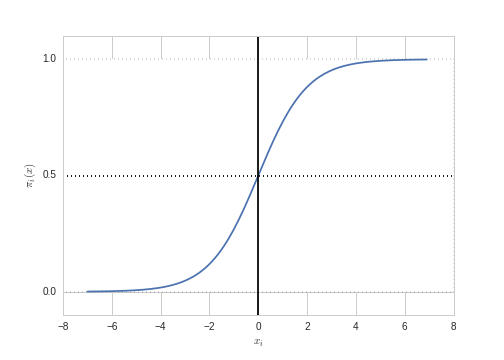
\includegraphics[scale=.75]{sigmoid.png}
\caption{The Sigmoidal Response Function. This function arises naturally for binary responses with values \{0,1\}. Pedro Domingos calls it "the most important curve in the world" in his recent book, The Master Algorithm.}
\label{fig:1}
\end{center}
\end{figure}
To perform feature selection we regularize the logistic regression model with an elastic net penalty. Under this particular approach, we find the model coefficients by maximizing the penalized logistic likelihood function:
\begin{equation} \label{eq:7}
\underset{\beta_{0k},\beta_k}{max} \Biggr\{\sum_{i=1}^N 
\left[ y_i\left( \beta_{0k}+\beta_k^T x_i \right) -\log \left( 1 + e^{\beta_{0k} + \beta_k^T x_i} \right) \right]-\lambda \sum_{k = 1}^K \sum_{j = 1}^p \left(\alpha\vert\beta_{kj}\vert\ +  \left(1-\alpha\right)\beta_{kj}^2\right) \Biggr\}.
\end{equation}
The second term of this energy is the elastic net penalty. The first sum in the penalty term operates over p-features for which we obtain p coefficients. The outer sum operates over K classes for which we would have K coefficient vectors, other than the intercept $\beta_0$. The first term inside this penalty imposes a sparse solution and the second term shrinks the coefficients of highly correlated features. In our particular case K=1 since we do not penalize the intercept $\beta_0$, and p varies depending on the class we analyze. Elastic net regularization is in a sense a combination of Tikhonov regularization \cite{tikhonov1963solution} and $L_1$ regularization \cite{tibshirani1996regression}. This method is particularly useful when $p>>n$ as it overcomes one of the drawbacks we encounter with $L_1$ regularization. If $p>n$, $L_1$ regularization (the LASSO) will only produce at most $n$ coefficients.
\subsection{Fitting the Regularized Logistic Model to the Breast Cancer Data}
We now fit the model by solving the likelihood maximization problem presented in equation (\ref{eq:7}) above. This is implemented using an open source machine learning learning library developed in the Python language called scikit-learn \cite{scikit-learn}. Sci-kit-learn uses the numerical technique Stochastic Gradient Descent to approximate the solution. We set the parameters $\lambda = 0.175$ and $\alpha = 0.5$.
\subsubsection{Monte Carlo Procedure for Variable Selection} \label{section:mc}
Given the relatively small number of samples, it is important not to over fit to this relatively small dataset. To accomplish this we use a basic Monte Carlo procedure:
\begin{itemize}
\item draw random samples from the original sample to create a training set;
\item fit the model on the training set and obtain model parameters;
\item apply the model on a test set to select the most significant genes;
\item repeat M times;
\item variables (significant genes) are selected based on overall selection frequency over all $M = 400$ trials, average p-values, and magnitude of coefficients.
\end{itemize}
The result of this procedure is summarized in table \ref{table:2}. The p-values in table \ref{table:2} are derived based on the Wald test on the following hypothesis:
\[H_0: \beta_k = 0\]
\[H_1: \beta_k \neq 0\]
with test statistic:
\[z=\frac{\hat{\beta_k}}{se\left(\hat{\beta_k}\right)}\sim N\left(0,1\right)\]
Clearly the first few coefficients in table \ref{table:2} are highly significant with very small p-values. The genes corresponding to these coefficients were selected by our algorithm in all but one trial. The model ends up selecting 1,182 genes. These are the genes in the model that have non-zero coefficients. However, we can affect this number by changing the tuning parameter $\alpha$ which is set at $0.5$. \\
\par Figure 2 shows the correlation structure among the first few genes which shows that the genes are correlated, perhaps highly. High correlation is a feature typical of gene expression data. The coefficients, however, have been shrunk by the penalty term in expression (\ref{eq:8}). Thus the estimated model corrects for the correlation among genes as in ridge regression. The elastic net regularized logistic regression estimates is then given by:
\begin{equation} \label{eq:8}
\boldsymbol{\hat{\beta}} = \text{arg max}\Biggr\{\sum_{i=1}^N 
\left[ y_i\left( \beta_{0k}+\beta_k^T x_i \right) -\log \left( 1 + e^{\beta_{0k} + \beta_k^T x_i} \right) \right]-\lambda \sum_{k = 1}^K \sum_{j = 1}^p \left(\alpha\vert\beta_{kj}\vert\ +  \left(1-\alpha\right)\beta_{kj}^2\right) \Biggr\}
\end{equation}
\par This solution is obtained numerically via Stochastic Gradient Descent.
\subsection{Choosing the Tuning Parameters, $\lambda$ and $\alpha$}
Choosing the tuning parameters is a key part of the fitting process. Essentially, $\lambda$ controls the magnitude of the penalty overall. Thus the higher the $\lambda$ the smaller the set of variables chosen by the model. Thus a balance must achieved between overfitting and underfitting the model. The parameter $\alpha$ strikes a balance between the LASSO penalty $\|\boldsymbol{\beta}\|_1$ and the ridge penalty $\|\boldsymbol{\beta}\|_2$. The LASSO penalty encourages a sparse solution by setting the coefficients of irrelevant genes to zero and the ridge penalty shrinks the coefficients of highly correlated genes towards each other, essentially forming "groups". \\
\par One criteria for choosing the tuning parameters is error rate (or conversely accuracy). The systematic selection of tuning parameters is achieved via cross-validation and selecting the parameters that provide the highest classification accuracy (or lowest classification error). Given the way we chose to evaluate and validate our model cross-validation on each of the validation trials (400 in total) proved to be computationally not feasible given our computing resources. As a result we chose a trial and error approach for $\lambda=\{0.1,0.125,0.150,0.175\}$ and $\alpha = 0.5$. The combination $\lambda = 0.175, \alpha = 0.5$ produced the highest mean accuracy and area under the ROC curve at $86\%$ and $84\%$ respectively.
\begin{table}
\begin{center}
\begin{tabular}{|c|c|c|c|c|}
\hline Gene & Frequency & Coefficient & Std-Error & p-value\\
\hline GI-4503602-S & 400 & 2.993167 & 0.7286791 & 1.998432e-05\\
\hline GI-38455428-S & 400 & 1.925685 & 0.6528698 & 0.001591082\\
\hline GI-29738585-S & 400 & 1.416221 & 0.4814823 & 0.001633779\\
\hline GI-21614543-S & 399 & -1.942821 & 0.6122178 & 0.000753285\\
\hline GI-9951924-S & 399 & 1.555703 & 0.5557352 & 0.002560192\\
\hline
\end{tabular}
\caption{The top five selected genes. We expect that the most significant genes are selected frequently, the absolute value of their coefficient is relatively large, and they are significant in terms of p-value.}
\label{table:2}
\end{center}
\end{table}

\begin{figure}[ht!]
\begin{center}
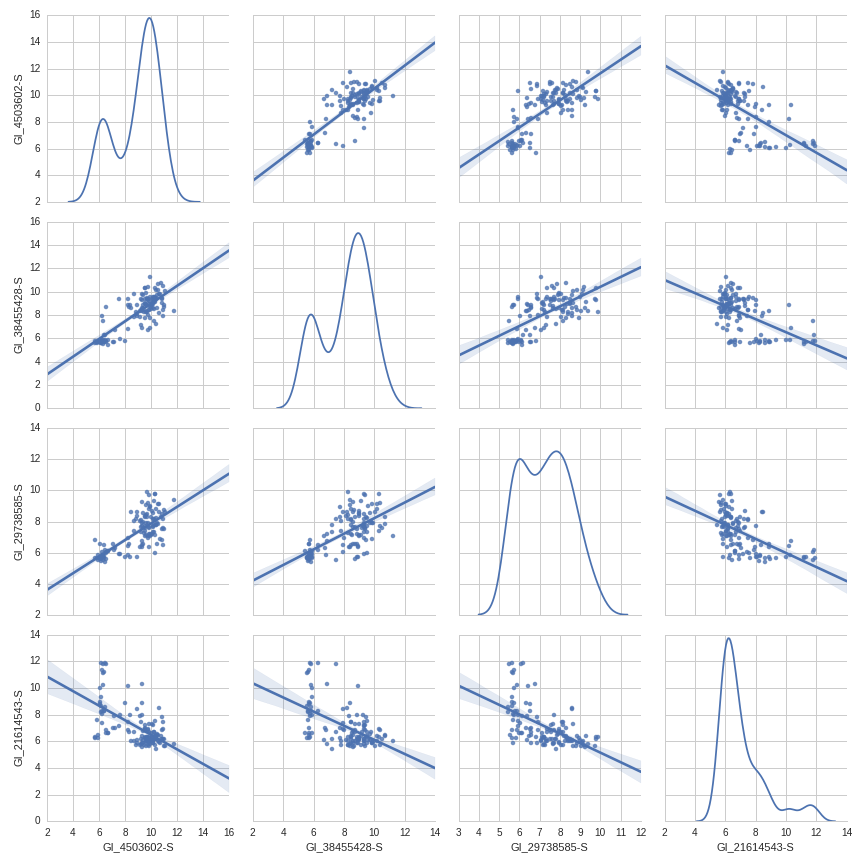
\includegraphics[scale=.4]{snscorr.png}
\caption{Correlation structure of the first four significant genes. The genes selected exhibit a non-trivial degree of correlation. This is expected as the  penalty term $\alpha \|\boldsymbol{\beta}\|_2$ allows the algorithm to select groups of genes that are correlated while shrinking their coefficient.}
\label{fig:2}
\end{center}
\end{figure}

\section{Model Evaluation }
\subsection{Evaluation Procedure}
In order to evaluate the model's performance we look at prediction accuracy. Too assess accuracy, we construct a procedure similar to the one described in section \ref{section:mc} but fit the model using only the 1,182 genes selected by the algorithm. As before, we split the data into a training set and a test set and calculate:
\begin{itemize}
\item the proportion of correct classifications (luminal vs. non-luminal) on the test set;
\item the confusion matrix;
\item the area under the receiver operating characteristic (ROC) curve.
\end{itemize}
We repeat this procedure $M = 400$ times and observe the mean accuracy result and mean area under the ROC curve. The ROC curve is a popular evaluation method for classifiers. It simply plots the True Positive Rate (TPR) vs. the False Positive Rate (FPR)as the as the threshold for classification is varied. For our regularized logistic classifier the threshold is based on the probability:
\[
P\left(Y=\text{luminal}|\text{Gene Expression}\right)
\]
The results obtained using this process are discussed below.
\subsection{Evaluation Results}
The resulting mean classification accuracy is 0.86 and the mean area under the ROC curve is 0.84 as shown in figure \ref{fig:3}. Given the complexity of the dataset, these results are encouraging. We were able to reduce the variable (genes) space from 47,293 to just over 1,000 genes, all while being able to classify cancer types correctly 86\% of the time.\\
\par Taking a closer look at the result, we see that the most significant gene identified in this analysis GI-4503602-S, which is the estrogen receptor 1. This particular gene has been identified by other studies as a highly explanatory genetic factor in breast cancer \cite{Glaab2012}. 
\begin{figure}[ht!]
\begin{center}
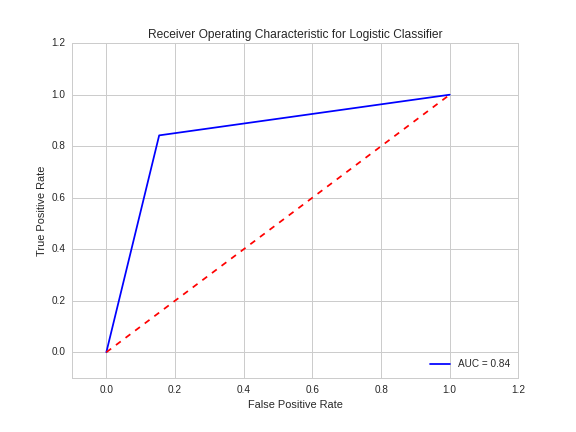
\includegraphics[scale=.625]{roc.png}
\caption{ROC curve for the Breast Cancer Logistic Classifier.}
\label{fig:3}
\end{center}
\end{figure}

\section{Conclusions}
The focus of this analysis is to tackle the issue analyzing high dimensional data. Specifically microarray gene expression data which typically has dimensions where $p>>n$. The proposed method for variable selection and dimensionality reduction: regularized logistic regression with the elastic net penalty, performed relatively well. It was able to reduce the dimensionality of the breast cancer gene expression dataset from 47,219 genes to just over 1,000. And based on this much smaller gene set we were able to classify cancer types with an approximate 86 percent accuracy. This methodology was enhanced repeated sampling validation in order to avoid overfitting to the data\\
\par Based on these results, the methodology presented here is a viable tools for researchers working with microarray data. However, it is important to compare and contrast this methodology with others. Classification, variable selection and dimensionality reduction are areas of active research and there exist many methodologies, such as Principal Component Analysis, Random Forests,a nd combinations thereof that we can use to the same end.\\
\par One of the nice features of penalized logistic regression is that first, it expresses the classification results as probabilities. Second, it is able to select more than $n$ variables, and last, it does not choose an arbitrary variable from a group of highly correlated variable. Rather, it chooses them all, albeit with "shrunk" coefficients - feature that is desirable in genomic expression analysis. \\
\par A question that must be raised in this analysis is whether the number of gene selected is the correct one? The variables selected in a sense are a function of the tuning parameters $\lambda$ and $\alpha$. We can use them as "valves" to turn the model's sensitivity up or down. Here we used trial and error to choose these tuning parameters according to the best classification accuracy we could find. In a future iteration, it would useful to explore more formal methods on how to choose these tuning parameters, an active area of research on its own right.
\ 
\FloatBarrier
\pagebreak
\section{Appendix: Python Code}
\subsection*{Data Cleaning}
\begin{verbatim}
# read data file
datafile = '~/Documents/THESIS/project/ICOS_DATA/breast_preprocessed.txt'
data = pd.read_table(datafile, delim_whitespace = True, 
                     dtype={'a': np.float64}, header = None)
                     
# data dimension
print data.shape
# last 5 rows of the data
data.tail()

# extract colum names (all but last one are gene names).
colNames = data[0]
colNames = list(colNames)

# tranpose the data to have genes as columns and microarray experiment as rows
data2 = data.T.ix[1:]

# reset the index to satrt at 0
data2 = data2.reset_index(drop=True)

# add colum labels
data2.columns=colNames

# create date set with genes only. This is the features matrix
X = data2[range(data.shape[0]-1)]
print X.shape

# make sure data type is float and not string.
X = X.astype(float)

# store the gene names/ids
geneNames = X.columns

# create vector with response variable
Y = data2[[-1]]

# make sure response vector is binary 0, 1.
Y = pd.get_dummies(Y)

# choose one of the equivalent response vectors.
Y = Y.ix[:,0]

#Percent of luminal.
np.mean(Y)
\end{verbatim}
\subsection{Model Fitting}
\begin{verbatim}
# model definition
# logistic regression with elasticnet regularization
# l1_ratio refers to alpha and alpha refers to lambda in Hastie
log_model = SGDClassifier(loss = 'log', penalty = 'elasticnet', alpha = 0.175, 
                                l1_ratio = 0.5, fit_intercept = True)
                                
#initialize the dataframes for ranking genes
selected_genes = {'col1':'gene1'}
gene_names = DataFrame(geneNames)
gene_names.columns = ['trial0']

# Initial trial column 
gene_select_count = gene_names.isin(selected_genes)
gene_coeff = DataFrame()

# Number of trials
M = 400

# IN THE LOOP
for i in range(M):
    # Split the data

    X_train, X_test, Y_train, Y_test = train_test_split(X, Y)


    # Fit model and select significant genes

    fit_log_model = log_model.fit(X_train, Y_train)
    X_selected = fit_log_model.transform(X_test)


    # Find the indexes of significant genes

    # these are the index of the features selected by the l1 regularized 
    # logistic model
    selected_index = np.where(log_model.coef_!=0)[-1]
    # Selected genes in ith trial
    selected_genes = gene_names.loc[selected_index]

    gene_select_count['trial' + str(i)] = gene_names.isin(selected_genes)
    gene_coeff['trial' + str(i)] = Series(log_model.coef_[0])
 
beta_coeff = gene_coeff.mean(axis = 1)
beta_sterror = gene_coeff.std(axis = 1)
gene_imp_score = gene_coeff.mean(axis = 1).abs()
pvalue = 1-norm.cdf(np.abs(beta_coeff/beta_sterror))

# this creates a pandas Series with the sum of how many times a gene was selected
gene_select_summary = gene_select_count.sum(axis = 1)

# this data frame has the values for all genes
result = DataFrame([geneNames, gene_select_summary, gene_imp_score, beta_coeff, 
beta_sterror, pvalue], index = 
          ['Gene', 'Frequency', 'Score', 'Coefficient', 'Std Error',            
          'pvalue']).T.sort(['Frequency', 'Score'], ascending = False)
          
# this gives the indices of selected genes according to some threshold. 
#can use the importance score
# or the number of times selected.
selected_genes_index = gene_select_summary[gene_imp_score >= 0.0000001].index

result = DataFrame([geneNames[selected_genes_index],
gene_select_summary[selected_genes_index], 
gene_imp_score[selected_genes_index], beta_coeff[selected_genes_index], 
beta_sterror[selected_genes_index],
pvalue[selected_genes_index]], index = ['Gene', 'Frequency', 'Score','Coefficient', 
'Std Error', 'pvalue']).T.sort(['Frequency', 'Score'], ascending = False)

result[['Gene', 'Frequency', 'Coefficient', 'Std Error', 'pvalue']]

# these are the names of the selected genes
DataFrame(geneNames[selected_genes_index], columns = ['Selected Genes'], 
index = selected_genes_index).head()
len(DataFrame(geneNames[selected_genes_index], columns = ['Selected Genes'], 
index = selected_genes_index))

#Need to create X_sel
X_sel = X[selected_genes_index]
\end{verbatim}
\subsection{Model Validation}
\begin{verbatim}

# Make a new log_model
#log_model2 = LogisticRegression()
log_model2 = LogisticRegression(dual = False, fit_intercept = True)

xvalacc = []
xvalROC = []
M = 400

for i in range(M):

    # Split the data
    X_train, X_test, Y_train, Y_test = train_test_split(X_sel, Y)

    # Now fit the new model
    log_model2.fit(X_train, Y_train)

    # Predict the classes of the testing data set
    class_predict = log_model2.predict(X_test)

    # Compare the predicted classes to the actual test classes
    xvalacc.append(metrics.accuracy_score(Y_test,class_predict))
    try:
        xvalROC.append(roc_auc_score(Y_test,class_predict))
    except ValueError:
        pass

np.mean(xvalacc)

np.mean(xvalROC)

confusion_matrix(Y_test,class_predict)

false_positive_rate, true_positive_rate, thresholds = roc_curve(Y_test,class_predict)

plt.title('Receiver Operating Characteristic')
plt.plot(false_positive_rate, true_positive_rate)
plt.legend(loc='lower right')
plt.plot([0,1],[0,1],'r--')
plt.xlim([-0.1,1.2])
plt.ylim([-0.1,1.2])
plt.ylabel('True Positive Rate')
plt.xlabel('False Positive Rate')
plt.show()   
\end{verbatim}
\pagebreak

\bibliographystyle{plain}
\bibliography{bibliography}

\end{document}